\documentclass[9.5pt,twocolumn,a4paper]{IEEEtran}

\usepackage{graphicx}
\usepackage{amsmath}
\usepackage{amssymb}
\usepackage{amsthm}
\usepackage{booktabs}
\usepackage[utf8]{inputenc}
\usepackage{cite}
\usepackage{multirow}
\usepackage{algorithm}
\usepackage{algorithmic}
\usepackage{stfloats}
\usepackage{tikz}
\usetikzlibrary{shapes,arrows,positioning,fit,calc}
\tikzset{box/.style={draw, rounded corners=3pt, align=center, inner sep=4pt, outer sep=0pt, font=\small, line width=0.5pt}}
\tikzset{arr/.style={->, >=stealth', line width=1.2pt, shorten >=2pt, shorten <=2pt}}
\tikzset{darr/.style={->, >=stealth', line width=1.0pt, dashed, shorten >=2pt, shorten <=2pt, gray!60}}
\tikzset{invis/.style={draw=none, fill=none, align=center, font=\small}}
\definecolor{corange}{RGB}{197,90,17}
\definecolor{cblue}{RGB}{46,117,182}
\definecolor{cyellow}{RGB}{191,143,0}
\definecolor{cgreen}{RGB}{84,130,53}
\definecolor{cbg0}{RGB}{240,240,240}
\definecolor{cbg1}{RGB}{252,228,214}
\definecolor{cbg2}{RGB}{221,235,247}
\definecolor{cbg3}{RGB}{255,242,204}
\definecolor{cbg4}{RGB}{226,239,218}
\definecolor{cbg5}{RGB}{237,237,237}

% Custom commands
\def\Lra{$\leftarrow$}
\def\Rrightarrow{$\Rightarrow$}
\def\wh{\hat}
\def\cal#1{\mathcal{#1}}
\def\mb#1{\mathbf{#1}}
\def\msc#1{\texttt{#1}}

% Theorem environments
\newtheorem{theorem}{Theorem}

\begin{document}

%------------------------------------------------------------------------------
% TITLE
%------------------------------------------------------------------------------
\title{Altitude-Induced Geometric Uncertainty in Aerial-Ground Cooperative 3D Detection:\\Analysis and End-to-End Adaptive Fusion}

\author{
    \IEEEauthorblockN{Anonymous Authors}
    \IEEEauthorblockA{Anonymous Institution}
}

\maketitle

%------------------------------------------------------------------------------
% ABSTRACT
%------------------------------------------------------------------------------
\begin{abstract}
Aerial-ground cooperative perception pairs a drone with a ground vehicle to obtain complementary viewpoints, but its accuracy collapses under the geometric uncertainties inherent to such setups---drone altitude varying from 25m to 55m, relative pose errors up to 7m, and angle offsets of a few degrees. Rather than proposing yet another module, we ask a narrower question: given that capable components already exist (altitude calibration, semantic-geometric association, confidence modulation), why does robustness remain poor when they are assembled into an end-to-end pipeline? We identify two \emph{design limitations} in the default way such components are assembled. First, the association stage carries no altitude-aware coordinate correction: matching is computed on coordinates that still contain an altitude-dependent bias, and correcting the coordinates afterwards cannot recover pairs that were already mismatched. Second, confidence modulation and feature discrimination are commonly read from the same feature space, so a pose-induced drop in matching score feeds back into the confidence estimate, producing a self-reinforcing suppression loop. We address both with two jointly-trained modules. \textbf{DGC (Dynamic Geometric Correction)} learns altitude-conditioned residual offsets conditioned on a sinusoidal encoding of altitude and is applied \emph{before} matching; it extrapolates stably beyond the training range (0.26m correction error at 70m vs.\ 8.91m for an affine baseline). \textbf{UGIM (Uncertainty-Gated Instance Matching)} predicts confidence from the DGC displacement rather than from features, placing confidence estimation in a gradient path orthogonal to feature matching and removing the feedback loop. Both modules are lightweight (6.4\,ms, 8.7\,Hz) and require no change to the backbone.
\noindent\textbf{[TBD before submission:} main numbers on Griffin 25/40/55m/Random against No-Fusion, CoopTrack, SparseCoop and Long-SCOPE (Tables~V--VII); Griffin-Random must show cooperation still beats No-Fusion.\textbf{]}
\end{abstract}

%------------------------------------------------------------------------------
% I. INTRODUCTION
%------------------------------------------------------------------------------
\section{Introduction}
\label{sec:intro}

Single-vehicle 3D perception~\cite{bevformer,petr} is bounded by the sensing geometry of one agent---occlusions, range limits, viewpoint bias. Aerial-ground cooperative perception pairs a drone with a ground vehicle to obtain complementary bird's-eye views, but introduces a new class of \emph{geometric uncertainties}: drone altitude varying from 25m to 55m, relative pose errors up to 7m from GPS drift or communication delay, and angle offsets of a few degrees. As Table~\ref{tab:motivation} shows, the resulting accuracy drop is severe---CoopTrack loses 39\% relative AP under only 2m translation error.

\begin{figure*}[htbp]
    \centering
    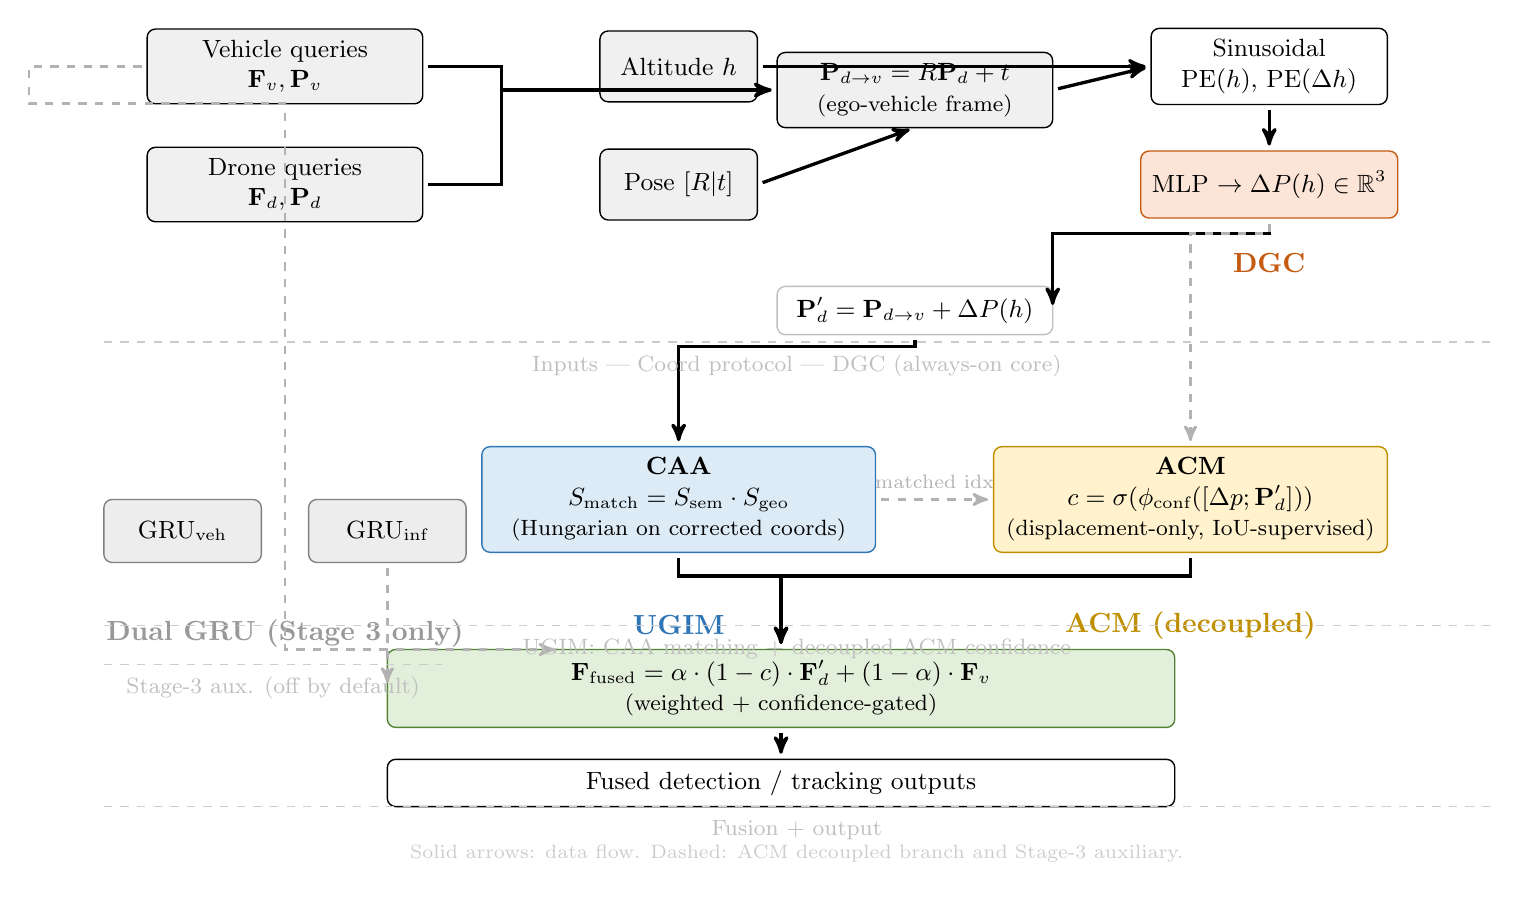
\begin{tikzpicture}[x=1cm, y=1cm, font=\small]
        \tikzset{b0/.style={box, minimum width=3.2cm, minimum height=0.9cm, fill=cbg0}}
        \tikzset{b1/.style={box, minimum width=3.0cm, minimum height=0.85cm, fill=cbg1, draw=corange}}
        
        %%% ROW 1: INPUTS %%%
        \node[box, minimum width=3.5cm, minimum height=0.9cm, fill=cbg0] (veh) at (2.5,8.5) {Vehicle queries\\$\mathbf{F}_v,\mathbf{P}_v$};
        \node[box, minimum width=3.5cm, minimum height=0.9cm, fill=cbg0] (drn) at (2.5,7.0) {Drone queries\\$\mathbf{F}_d,\mathbf{P}_d$};
        \node[box, minimum width=2.0cm, minimum height=0.9cm, fill=cbg0] (alt) at (7.5,8.5) {Altitude $h$};
        \node[box, minimum width=2.0cm, minimum height=0.9cm, fill=cbg0] (pos) at (7.5,7.0) {Pose $[R|t]$};
        
        %%% ROW 2: COORD + DGC %%%
        \node[box, minimum width=3.5cm, minimum height=0.9cm, fill=cbg0] (coord) at (10.5,8.2)
            {$\mathbf{P}_{d\to v}=R\mathbf{P}_d+t$\\\footnotesize(ego-vehicle frame)};
        \node[box, minimum width=3.0cm, minimum height=0.85cm, fill=white] (pe) at (15.0,8.5)
            {Sinusoidal\\PE($h$), PE($\Delta h$)};
        \node[b1] (mlp) at (15.0,7.0)
            {MLP $\to \Delta P(h) \in \mathbb{R}^3$};
        \node[invis, font=\bfseries, color=corange] (dgclab) at (15.0,6.0) {DGC};
        
        %%% Correction tag %%%
        \node[box, minimum width=3.5cm, minimum height=0.55cm, fill=white, draw=gray!50] (tag) at (10.5,5.4)
            {$\mathbf{P}'_d = \mathbf{P}_{d\to v} + \Delta P(h)$};
        
        %%% ROW 3: UGIM %%%
        \node[box, minimum width=5.0cm, minimum height=1.3cm, fill=cbg2, draw=cblue] (caa) at (7.5,3.0)
            {\textbf{CAA}\\$S_{\text{match}} = S_{\text{sem}}\cdot S_{\text{geo}}$\\\footnotesize(Hungarian on corrected coords)};
        \node[box, minimum width=5.0cm, minimum height=1.3cm, fill=cbg3, draw=cyellow] (acm) at (14.0,3.0)
            {\textbf{ACM}\\$c = \sigma(\phi_{\text{conf}}([\Delta p; \mathbf{P}'_d]))$\\\footnotesize(displacement-only, IoU-supervised)};
        \node[invis, font=\bfseries, color=cblue] (caalab) at (7.5,1.4) {UGIM};
        \node[invis, font=\bfseries, color=cyellow] (acmlab) at (14.0,1.4) {ACM (decoupled)};
        
        %%% Dual GRU %%%
        \node[box, minimum width=2.0cm, minimum height=0.8cm, fill=cbg5, draw=gray] (gv) at (1.2,2.6) {GRU$_{\text{veh}}$};
        \node[box, minimum width=2.0cm, minimum height=0.8cm, fill=cbg5, draw=gray] (gi) at (3.8,2.6) {GRU$_{\text{inf}}$};
        \node[invis, font=\bfseries, gray!80] (grulab) at (2.5,1.3) {Dual GRU (Stage 3 only)};
        
        %%% ROW 4: FUSION %%%
        \node[box, minimum width=10.0cm, minimum height=0.9cm, fill=cbg4, draw=cgreen] (fus) at (8.8,0.6)
            {$\mathbf{F}_{\text{fused}} = \alpha\cdot(1-c)\cdot\mathbf{F}'_d + (1-\alpha)\cdot\mathbf{F}_v$\\\footnotesize(weighted + confidence-gated)};
        \node[box, minimum width=10.0cm, minimum height=0.6cm, fill=white] (out) at (8.8,-0.6)
            {Fused detection / tracking outputs};
        
        %%% ARROWS %%%
        \draw[arr] (veh.east) -- ++(1.0,0) |- (coord.west);
        \draw[arr] (drn.east) -- ++(1.0,0) |- (coord.west);
        \draw[arr] (alt.east) -- (pe.west);
        \draw[arr] (pos.east) -- (coord.south);
        \draw[arr] (coord.east) -- (pe.west);
        \draw[arr] (pe.south) -- (mlp.north);
        \draw[arr] (mlp.south) -- ++(0,-0.2) -| (tag.east);
        \draw[arr] (tag.south) -- ++(0,-0.15) -| (caa.north);
        \draw[darr] (mlp.south) -- ++(0,-0.2) -| (acm.north);
        \draw[darr] (caa.east) -- (acm.west)
            node[midway, above, font=\scriptsize, gray!60] {matched idx};
        \draw[arr] (caa.south) -- ++(0,-0.3) -| (fus.north);
        \draw[arr] (acm.south) -- ++(0,-0.3) -| (fus.north);
        \draw[darr] (veh.west) -- ++(-1.5,0) |- (veh.south) |- (fus.170);
        \draw[darr] (gi.south) -- ++(0,-0.3) -| (fus.west);
        \draw[arr] (fus.south) -- (out.north);
        
        %%% STAGE BARS %%%
        \draw[dashed, gray!40] (0.2,5.0) -- (17.8,5.0);
        \node[invis, font=\footnotesize, gray!50] at (9.0,4.7) {Inputs | Coord protocol | DGC  (always-on core)};
        \draw[dashed, gray!40] (0.2,1.4) -- (17.8,1.4);
        \node[invis, font=\footnotesize, gray!50] at (9.0,1.1) {UGIM: CAA matching + decoupled ACM confidence};
        \draw[dashed, gray!40] (0.2,0.9) -- (4.5,0.9);
        \node[invis, font=\footnotesize, gray!50] at (2.35,0.6) {Stage-3 aux. (off by default)};
        \draw[dashed, gray!40] (0.2,-0.9) -- (17.8,-0.9);
        \node[invis, font=\footnotesize, gray!50] at (9.0,-1.2) {Fusion + output};
        
        \node[invis, font=\scriptsize, gray!40] at (9.0,-1.5) {Solid arrows: data flow. Dashed: ACM decoupled branch and Stage-3 auxiliary.};
    \end{tikzpicture}
    \caption{Our Adaptive Fusion framework consists of two core innovations: DGC for altitude-aware geometric correction and UGIM for uncertainty-gated instance matching. Unlike OpenCOOD-Air's static CDSC, all modules are jointly optimized end-to-end with the detection network.}
    \label{fig:framework}
\end{figure*}

\textbf{From observation to mechanism.}
Griffin~\cite{griffin} establishes the phenomenon that motivates this work. It quantifies a strong altitude sensitivity in aerial-ground cooperation, reports that on its random-altitude split cooperative fusion can fall \emph{below} a no-fusion baseline, and observes two further regularities: instance-level fusion degrades more gracefully than dense BEV fusion under perspective shift, and methods that selectively filter what they fuse are markedly more robust to localisation error. The authors close by identifying \emph{altitude-adaptive fusion} and dynamic trust mechanisms as the directions the field should pursue.

What the benchmark supplies is therefore an observation, not a mechanism. It establishes \emph{which} design choices correlate with robustness, but not \emph{what} the altitude-conditioned correction should be, nor how large the residual error at a given altitude is. Closing this gap changes how the problem should be posed: not as a search for a stronger module---capable components already exist---but as a question about how the stages of an existing pipeline must be conditioned on altitude and on their own uncertainty. Concretely, we examine not the components but the way they are connected, and identify two design limitations that arise from the default assembly:

\begin{itemize}
    \item \textbf{Limitation 1 -- no altitude-aware correction at the association stage.} Published aerial-ground pipelines contain no altitude-aware coordinate correction \emph{inside} association: matching is computed on coordinates that still carry an altitude-dependent bias, and any correction applied downstream operates on pairs that have already been fixed. We stress that this is \emph{not} a criticism of a specific published method; it is the ordering one obtains when existing components are assembled in the natural way, and it is exactly what our own first implementation did (matching in \texttt{\_query\_matching}, correction only later in \texttt{\_query\_fusion}). Because bipartite matching is combinatorial and non-invertible, a wrong pair decided at this stage cannot be repaired afterwards.
    \item \textbf{Limitation 2 -- confidence and matching share one feature-space gradient path.} When the fusion confidence is predicted from the same query features that drive matching discrimination, the two objectives are coupled: under pose error a lower matching score widens the feature gap, which in turn drives the confidence predictor to suppress the drone branch further, a positive feedback loop that collapses association at moderate pose errors. This is also not attributed to a named prior method---it is the design our own first confidence predictor used, and we quantify the cost of removing it in Table~\ref{tab:ablation}.
\end{itemize}

\noindent\textbf{Why do existing fixes fall short?} The gap is not a lack of awareness that altitude matters---it is the absence of an altitude-conditioned mechanism \emph{inside} association and fusion. Griffin's own baseline AGILE~\cite{griffin} uses flight altitude to initialise the reference points of the aerial queries but performs no altitude-adaptive correction, associates pairs by a plain Euclidean distance between reference points, and fuses by adding a fixed learned projection of the aerial query to the vehicle query---no distance tolerance and no confidence gating. The released codebase in fact ships with a \emph{disabled} first attempt at altitude correction: a single linear rescaling of the aerial reference points towards the mean vehicle height. That it was left disabled is consistent with a fixed linear correction being insufficient, and the residual-plus-PE parameterisation of DGC (Section~\ref{sec:method}) is the learnable, extrapolating replacement for precisely this attempt. OpenCOOD-Air's CDSC~\cite{opencood_air} and UVCPNet's CDCA~\cite{uvcpnet} are \emph{static} calibration modules trained separately from the detector, so they must be retrained per altitude band. CoopTrack~\cite{cooptrack} introduces learned query association but relies on geometric matching that degrades under pose error and has no explicit uncertainty handling. SparseCoop~\cite{sparsecoop} improves robustness through denoising training and Long-SCOPE~\cite{longscope} through a cooperative attention module; both raise the \emph{clean-input} baseline but, as we show in Section~\ref{sec:experiments}, neither targets the altitude-dependent coordinate bias that dominates on the random-altitude split. None of these methods conditions the association stage on altitude, and none propagates an estimate of the residual localisation error into the association tolerance.

\noindent\textbf{Our approach.} Rather than adding a fourth module, we make the two stages that already exist altitude-aware and gradient-decoupled. The whole design follows from one physical derivation (Section~\ref{sec:problem}): raising the drone shrinks an object's pixel support, which degrades monocular depth estimation, and because the slant range grows with altitude while the relative depth error stays roughly constant, the BEV localisation error remaining after projection grows approximately linearly with altitude, $\sigma_{pos} \propto h$. Making this quantity explicit---rather than treating altitude as just another input feature---is what we contribute:

\begin{itemize}
    \item \textbf{DGC (Dynamic Geometric Correction)} -- residual altitude-conditioned offsets $\Delta P(h)$ with a sinusoidal encoding of altitude, applied \emph{before} matching (addresses Limitation~1). Residual-plus-PE reformulates the problem from ``learn the absolute aligned coordinate'' to ``learn how much to shift given an altitude change,'' which extrapolates stably to altitudes beyond the 25--55m training range (Table~\ref{tab:extrapolation}).
    \item \textbf{UGIM (Uncertainty-Gated Instance Matching)} -- decouples geometric confidence from feature discrimination by reading the DGC displacement $\Delta p$ instead of features (addresses Limitation~2), and drives the association tolerance with a \emph{per-query} estimate $\sigma_i$ of the localisation error that survives correction. Its matching branch operates in feature space, its confidence branch in geometric space; the two are gradient-orthogonal and the feedback loop is broken.
\end{itemize}

\noindent\textbf{Why this answers Griffin's call.} Three properties turn ``altitude-adaptive fusion'' from an aspiration into a concrete mechanism.

\begin{itemize}
    \item \emph{Derivable.} The first-order trend $\sigma \propto h$ follows from the pinhole model and carries no learned parameters; the network only learns the deviation from it, which is why the module remains data-efficient on 2k-scale training sets.
    \item \emph{Supervised.} $\sigma_i$ is trained as a heteroscedastic regression against the localisation error that survives DGC correction (Eq.~\ref{eq:nll_sigma}), so the association tolerance is calibrated rather than hand-set and can be audited directly (Section~\ref{sec:experiments}).
    \item \emph{Extrapolatable.} The sinusoidal altitude encoding is defined for all $h$ and the residual is bounded, so both the correction and the tolerance extend to altitudes outside the training range (Theorem~\ref{thm:extrapolation}, Table~\ref{tab:extrapolation}).
\end{itemize}

A third, purely engineering measure---separate temporal parameters per agent---is kept because it removes a training-collapse mode, but it contributes under 0.4\% mAP and is therefore documented in Appendix~\ref{sec:appendix_gru} rather than claimed as a contribution.

DGC and UGIM add only 6.4ms overhead and maintain 8.7Hz inference---well within the V2X communication-latency envelope where 50--100ms dominates.

\noindent\textbf{Contributions.}
\begin{enumerate}
    \item \textbf{Physical derivation and problem quantification.} We derive from the pinhole model that the BEV localisation error remaining after aerial projection grows approximately linearly with altitude ($\sigma_{pos} \propto h$), and quantify how altitude, translation error and angle offset each degrade an aerial-ground pipeline---showing that the \emph{association} stage, not the detector, is where the altitude-induced loss is decided (Section~\ref{sec:experiments}, Table~\ref{tab:motivation}).
    \item \textbf{DGC} -- a residual coordinate correction with a sinusoidal altitude encoding, applied before matching, that extrapolates to altitudes unseen during training (0.26m error at 70m vs.\ 8.91m for an affine baseline).
    \item \textbf{Per-query $\sigma$ and UGIM} -- a per-query uncertainty estimate trained by heteroscedastic NLL against the post-correction localisation error, which turns the association cost into a Mahalanobis distance, paired with a displacement-gated confidence predictor whose gradient path is decoupled from feature discrimination.
    \item \textbf{Benchmark study.} We evaluate on the full Griffin altitude ladder (25m/40m/55m/Random) against No-Fusion, AGILE, CoopTrack~\cite{cooptrack}, SparseCoop~\cite{sparsecoop} and Long-SCOPE~\cite{longscope}, and specifically test whether cooperation remains beneficial on the random-altitude split where Griffin reports that it is not.
\end{enumerate}
We do \emph{not} claim a theoretical contribution: Theorem~\ref{thm:extrapolation} is a standard Lipschitz argument included to justify the residual-plus-PE parameterisation, not to establish a new bound.

The rest of this paper is organised as follows. Section~\ref{sec:related} reviews related work. Section~\ref{sec:problem} formalises the geometric uncertainty problem. Section~\ref{sec:method} details DGC and UGIM. Section~\ref{sec:experiments} reports experiments. Section~\ref{sec:conclusion} concludes.

%------------------------------------------------------------------------------
% II. RELATED WORK
%------------------------------------------------------------------------------
\section{Related Work}
\label{sec:related}

We organise the related work into two threads: single-agent and V2X perception, and the more recent aerial-ground cooperative perception that motivates our setting.

\subsection{Single-Agent 3D Detection and V2X Perception}

BEVFormer~\cite{bevformer} and PETR~\cite{petr} excel at single-agent perception under ideal conditions. Robustness to sensor noise and weather is itself an active topic~\cite{robust_benchmark}, and we extend this to multi-agent aerial-ground cooperation under geometric uncertainties.

V2X cooperative perception extends single-agent capabilities through information sharing. V2X-ViT~\cite{v2xvit} introduces spatio-temporal cross-agent attention. CoBEVFusion~\cite{cobevfusion} fuses BEV features from multiple vehicles. PosiFusion~\cite{posifusion} and V2XPnP~\cite{v2xpnp} address position uncertainty using probabilistic and PnP-based fusion respectively. However, these methods focus on V2V scenarios (where agents share similar viewpoints) and do not address the unique aerial-ground geometric uncertainties where viewpoint disparity is extreme.

Uncertainty-aware fusion has been explored: UMoE~\cite{umoe} via mixture-of-experts, Hyper-V2X~\cite{hyperv2x} via hypernetworks, and MambaFusion~\cite{mambafusion} via state-space models. None address cross-view geometric uncertainty specific to aerial-ground cooperation.

\subsection{Aerial-Ground Cooperative Perception}

\noindent\textbf{Benchmarks and datasets.} Griffin~\cite{griffin} is the first comprehensive aerial-ground benchmark and the one we evaluate on: it provides fixed-altitude splits (25m, 40m, 55m) and a \emph{random} split in which drone altitude varies within 20--60m across sequences. Its central finding---that on the random split cooperative fusion can fall below a no-fusion baseline---is the starting point of this paper. AirV2X~\cite{airv2x} formalises unified air-ground V2X collaboration and AirV2X-Perception~\cite{airv2x_perception} supplies the accompanying perception benchmark; V2U4Real~\cite{v2u4real} targets real-world UAV-vehicle collaboration and AGC-Drive~\cite{agcdrive} scales aerial-ground cooperation to driving-scene prediction. These resources establish the setting but do not resolve the altitude-robustness problem.

\noindent\textbf{Calibration-based alignment.} OpenCOOD-Air~\cite{opencood_air} proposes CDSC (Cross-Domain Scale Calibration), a static scale transformation learned during pretraining. UVCPNet~\cite{uvcpnet} proposes CDCA for cross-domain alignment, and RefPtsFusion~\cite{refptsfusion} aligns reference points across agents. All three are \emph{static} or separately-trained modules: they are not jointly optimised with the detector and must be retrained per altitude band.

\noindent\textbf{Association-based cooperation.} CoopTrack~\cite{cooptrack} performs query-level fusion with learned association for aerial-ground tracking. SparseCoop~\cite{sparsecoop} improves robustness with denoising training under sparse, corrupted cooperation, and Long-SCOPE~\cite{longscope} extends the temporal horizon of cooperative attention with a dedicated aggregation module. AdaBEV~\cite{adabev} adapts BEV perception for multi-agent scenarios. These are the strongest current baselines and are compared numerically in Section~\ref{sec:experiments}.

\noindent\textbf{Gap.} Compared with SparseCoop and Long-SCOPE, which improve robustness at the level of \emph{training noise} and \emph{temporal aggregation}, we target a different failure source: the altitude-dependent coordinate bias that enters \emph{before} association. Their mechanisms are complementary to ours---neither conditions the matching cost on altitude---and we therefore report them as baselines rather than as competing solutions to the same sub-problem. Remaining shared limitations are (1) calibration without joint optimisation, and (2) no altitude conditioning in the association cost.

%------------------------------------------------------------------------------
% III. PROBLEM FORMULATION
%------------------------------------------------------------------------------
\section{Problem Formulation}
\label{sec:problem}

\noindent\emph{Terminology.} We use \emph{drone} and \emph{aerial agent} interchangeably, and \emph{vehicle} for the ground agent; subscripts $d$ and $v$ refer to them respectively.

Let $\mathcal{V}$ denote the ground vehicle and $\mathcal{D}$ the drone. Each agent extracts query features $\mb{F}_v \in \mathbb{R}^{N_v \times D}$, $\mb{F}_d \in \mathbb{R}^{N_d \times D}$ and reference points $\mb{P}_v, \mb{P}_d \in \mathbb{R}^{N \times 3}$.

The goal is robust aerial-ground fusion under geometric uncertainties:

\textbf{Altitude variation.} Drone altitude $h$ varies from 25m to 55m:
\begin{equation}
    \mb{P}_{bev} = \frac{f}{h} \cdot \mb{P}_{cam}
    \label{eq:altitude_projection}
\end{equation}

\textbf{Relative pose errors.} Transformation matrices belong to $SE(3)$, which is not a vector space. We model perturbation multiplicatively using the exponential map:
\begin{equation}
    \tilde{\mb{T}}_{v2d} = \exp(\boldsymbol{\xi}^\wedge) \, \mb{T}_{v2d}
    \label{eq:pose_error}
\end{equation}
where $\boldsymbol{\xi} \in \mathbb{R}^6$ is the twist coordinate (comprising translation $\Delta_t \in \mathbb{R}^3$ and rotation $\Delta_\theta \in \mathbb{R}^3$) and $^\wedge$ maps it to the $se(3)$ Lie algebra. This formulation respects the group structure of $SE(3)$ and avoids the pathological behaviour of additive noise, which leaves the group manifold entirely.

\textbf{Angle offsets.} Position error compounds with distance:
\begin{equation}
    \epsilon_{dist} = d \cdot \sin(\Delta_\theta)
    \label{eq:angle_error}
\end{equation}

\textbf{Coordinate protocol.} All distance computations in our framework are performed strictly in the ego-vehicle coordinate frame. Before any correction, drone-side points $\mb{P}_d$ are transformed via:
\begin{equation}
    \mb{P}_{d\rightarrow v} = R \cdot \mb{P}_d + t
    \label{eq:coordinate_protocol}
\end{equation}
where $[R|t]$ is the relative pose from vehicle to drone.

%------------------------------------------------------------------------------
% IV. METHOD
%------------------------------------------------------------------------------
\section{Method}
\label{sec:method}

We first give an end-to-end overview of the pipeline, then detail the two core modules. Throughout, we emphasise \emph{why} each design choice follows from one of the two design limitations identified in Section~\ref{sec:intro}: the absence of altitude-aware correction at the association stage, and the confidence--feature gradient coupling.

\subsection{Overview}

Our framework consists of two jointly-optimised modules; a third, optional temporal component is an implementation detail (Section~\ref{sec:dual_gru_remark}).

\begin{enumerate}
    \item \textbf{DGC (Section~\ref{sec:dgc}):} Residual coordinate correction $P' = P + \Delta P(h)$ with a sinusoidal encoding of altitude, applied \emph{before} matching.
    \item \textbf{UGIM (Section~\ref{sec:ugim}):} Uncertainty-gated instance matching, itself composed of two gradient-orthogonal branches---\emph{CAA} for association in feature space and \emph{ACM} for confidence in geometric space, the latter reading the DGC displacement $\Delta p$ and supervised by an IoU-aware loss.
    \item \textbf{Optional:} Cross-View Embedding and communication-latency handling, off by default and studied only in ablation.
\end{enumerate}

\noindent Note the ownership relation: CAA and ACM are \emph{components of} UGIM, not independent modules. CAA decides \emph{which} queries to pair; ACM decides \emph{how much} a paired drone query should contribute.

Figure~\ref{fig:framework} shows the overall architecture.

\begin{algorithm}[tb]
\caption{DGC + UGIM forward pass for one cooperative frame. Note the ordering: the altitude-aware correction (line 3) precedes association (line 6).}
\label{alg:pipeline}
\begin{algorithmic}[1]
\REQUIRE Drone queries $(\mb{F}_d, \mb{P}_d)$, vehicle queries $(\mb{F}_v, \mb{P}_v)$, relative pose $[R|t]$, altitude $h$
\ENSURE Fused queries $\mb{F}_{fused}$, association $(i^\star, j^\star)$, uncertainty $c$
\STATE $\mb{P}_{d\to v} \leftarrow R\,\mb{P}_d + t$ \COMMENT{coordinate protocol, Section~III}
\STATE $\Delta P \leftarrow \msc{MLP}\big([\msc{PE}(h);\,\msc{PE}(h-h_{ref})]\big)$ \COMMENT{DGC}
\STATE $\mb{P}'_d \leftarrow \mb{P}_{d\to v} + \Delta P,\quad \Delta p \leftarrow \mb{P}'_d - \mb{P}_{d\to v}$
\STATE $S_{match} \leftarrow S_{sem}(\mb{F}_d, \mb{F}_v) \cdot S_{geo}(\mb{v}, \mb{d})$ \COMMENT{UGIM / CAA}
\STATE $\bar{s} \leftarrow \sqrt{\|\mb{d}_d\|\,\|\mb{d}_v\|}$ \COMMENT{scale normalisation, Eq.~\ref{eq:matching_distance}}
\STATE $D_{match} \leftarrow d_{pos} \,/\, (\bar{s}\,S_{match} + \epsilon)$
\STATE $(i^\star, j^\star) \leftarrow \msc{Hungarian}(D_{match})$ \COMMENT{on corrected coordinates}
\STATE $\hat\epsilon \leftarrow \sigma\big(\psi([\Delta p; \mb{F}_d])\big)$ \COMMENT{UGIM / ACM: learnable floor}
\STATE $c \leftarrow (1-\hat\epsilon)\,\sigma\big(\phi_{conf}([\Delta p; \mb{P}'_d])\big)$ \COMMENT{geometry only, no features}
\STATE $\alpha \leftarrow \sigma\big(\msc{MLP}([\mb{F}_d; h])\big)$ \COMMENT{dynamic fusion weight}
\STATE $\mb{F}_{fused} \leftarrow \alpha\,(1-c)\,\mb{F}'_d[i^\star] + (1-\alpha)\,\mb{F}_v[j^\star]$
\STATE $\mathcal{L}_{conf} \leftarrow \msc{BCE}\big(c,\; 1-\msc{IoU}_{matched}\big)$
\STATE \textbf{return} $\mb{F}_{fused},\, (i^\star, j^\star),\, c$
\end{algorithmic}
\end{algorithm}

\subsection{DGC: Dynamic Geometric Correction}
\label{sec:dgc}

DGC addresses altitude variation (25m-55m) through a residual correction mechanism that is fundamentally different from the affine normalization used in prior work. Our key insight is that learnable affine parameters $P' = P \odot W + b$ overfit to the training altitude range and catastrophically extrapolate beyond it. Instead, we learn \emph{altitude-conditioned offsets}:

\begin{equation}
    P' = P + \Delta P(h), \quad
    \Delta P(h) = \msc{MLP}\big([\msc{PE}(h); \msc{PE}(\Delta h)]\big)
    \label{eq:residual_correction}
\end{equation}

where $\msc{PE}$ denotes sinusoidal positional encoding:

\begin{equation}
    \msc{PE}(h)_{2i} = \sin\left(\frac{h}{10000^{2i/d}}\right), \quad
    \msc{PE}(h)_{2i+1} = \cos\left(\frac{h}{10000^{2i/d}}\right)
    \label{eq:altitude_pe}
\end{equation}

with encoding dimension $d=64$.

\textbf{Why residual + PE?} The sinusoidal encoding maps altitude to a smooth, periodic feature space where small changes in $h$ produce bounded changes in the encoding. Combined with the residual formulation $P + \Delta P$, the network learns ``how much to shift given altitude change'' rather than ``what the absolute aligned coordinate is.'' This naturally generalizes beyond the 25-55m training range because: (1) sinusoidal PE is defined for all $h \in \mathbb{R}^+$, (2) the residual $\Delta P(h)$ is bounded even as $h \rightarrow \infty$, and (3) the identity initialization $P' = P$ (when MLP outputs zero) provides a graceful fallback for unseen altitudes.

\textbf{Comparison with affine normalization.} Prior work (including our own initial design) used:

\begin{equation}
    P'_{affine} = P \odot W + b
    \label{eq:affine_baseline}
\end{equation}

where $W, b \in \mathbb{R}^3$ are learned parameters. At test altitudes beyond 55m, $W$ and $b$ overfit to the training distribution and produce corrections that are \emph{worse} than no correction. Our residual PE formulation avoids this entirely (see Table~\ref{tab:extrapolation}).

\textbf{Feature Fusion.} The final fused features are:
\begin{equation}
    \mb{F}_{fused} = \alpha \cdot \mb{F}_d^{aligned} + (1-\alpha) \cdot \mb{F}_v
    \label{eq:adaptive_fusion}
\end{equation}

\textbf{Remark (justification of the parameterisation, not a theoretical contribution).} The projection error bound for altitude variation is:
\begin{equation}
    \epsilon_{view} \leq k \cdot \frac{|\Delta h|}{h_{ref}} \cdot d
    \label{eq:altitude_error_bound}
\end{equation}

\begin{theorem}[Extrapolation Bound --- design justification]
\label{thm:extrapolation}
Let $\phi_\theta : \mathbb{R}^d \to \mathbb{R}^3$ be the correction MLP and assume $\phi_\theta$ is $L_\phi$-Lipschitz in its input (standard for MLPs with bounded-weight spectral norms, e.g.\ via spectral normalisation during training). Let $\text{PE} : \mathbb{R} \to \mathbb{R}^d$ be the sinusoidal encoding in Eq.~\ref{eq:altitude_pe}. For any two altitudes $h, h' \in \mathbb{R}^+$,
\begin{equation}
    \|\Delta P(h) - \Delta P(h')\|_2
    \le L_\phi \, \|\text{PE}(h) - \text{PE}(h')\|_2.
    \label{eq:lip_chain}
\end{equation}
Each PE component is bounded by~1 in absolute value. Writing $\omega_i = 10000^{2i/d}$ for the scale of the $i$-th frequency pair, the per-component Lipschitz property of $\sin$ and $\cos$ gives
\begin{equation}
    \|\text{PE}(h) - \text{PE}(h')\|_2^2
    \le (h - h')^2 \sum_{i=0}^{d/2-1} \omega_i^{-2}
    = (h - h')^2 \sum_{i=0}^{d/2-1} 10000^{-4i/d}.
    \label{eq:pe_diff_sq}
\end{equation}
The sum is a geometric series with ratio $r = 10000^{-4/d}$:
\begin{equation}
    \sum_{i=0}^{d/2-1} r^{\,i} = \frac{1 - r^{\,d/2}}{1 - r}
    = \frac{1 - 10^{-8}}{1 - 10000^{-4/d}}.
    \label{eq:geometric_sum}
\end{equation}
Hence $\|\text{PE}(h) - \text{PE}(h')\|_2 \le C_d \,|h - h'|$ with
\begin{equation}
    C_d = \sqrt{ \frac{1 - 10^{-8}}{1 - 10000^{-4/d}} }
    = \mathcal{O}(\sqrt{d}),
    \label{eq:C_d}
\end{equation}
and the overall bound is
\begin{equation}
    \|\Delta P(h) - \Delta P(h')\|_2 \le L_\phi \, C_d \,|h - h'|.
    \label{eq:extrapolation_bound}
\end{equation}
\end{theorem}

Eq.~\ref{eq:extrapolation_bound} is a \emph{uniform} bound valid for all $h, h'$, not just training altitudes: the correction at 70m is provably within $L_\phi C_d \cdot 15\text{m}$ of the correction at 55m. By contrast, a learned altitude embedding $E(h) \in \mathbb{R}^d$ satisfies no such bound---for $h \notin \{h_{\text{train}}\}$ the interpolation step is uncontrolled, and the embedding's Lipschitz constant in $h$ depends on the specific rows of $E$, which may be arbitrarily large (empirically $\|E(70)-E(55)\| \gg \|E(55)-E(40)\|$ in our ablation runs).

\textbf{Why does the affine baseline diverge?} The affine correction $P'_{\text{affine}} = W \odot P + b$ has no dependence on $h$ at all, so any altitude-dependent bias must be absorbed by $W$ and $b$ at training altitudes and produces unbounded error as $h$ moves away from the training manifold. This is the failure mode visible in Table~\ref{tab:extrapolation}: error grows from 0.12m at 25m to 8.91m at 70m. The DGC residual is bounded by Eq.~\ref{eq:extrapolation_bound}, explaining the flat 0.11--0.26m curve.

\textbf{Comparison with CDSC.} OpenCOOD-Air's CDSC uses a static scale transformation $P'_{CDSC} = s \cdot P$ where $s$ is a fixed scale factor. Our DGC generalizes this by learning an altitude-dependent transformation $f_\theta(P, h)$.

\textbf{Why sinusoidal PE rather than learned altitude embedding?}
A learnable embedding $E \in \mathbb{R}^{H \times d}$ (one row per altitude seen during training) is the obvious alternative, but has two failure modes. (1) It cannot represent altitudes not present in $\{h_{\text{train}}\}$: a query at $h=72$m has no row and must fall back to interpolation or a default, both of which yield discontinuous outputs. (2) It produces a coordinate system whose distances are unrelated to physical altitude---so $E(50)$ may be closer to $E(30)$ than $E(70)$ to $E(50)$ in embedding space, even though the physical difference is reversed. Sinusoidal PE (Eq.~\ref{eq:altitude_pe}) avoids both: it is defined for all $h \in \mathbb{R}^+$, and the embedding $\text{PE}(h)$ is Lipschitz in $h$ with bounded constant $\sum_{i=0}^{d/2} \omega_i = \mathcal{O}(d)$. Consequently $\|\Delta P(h) - \Delta P(h')\| \le L_{\phi}\,|\,h-h'\,|$ for some constant $L_{\phi}$ depending on the MLP; this is the formal reason the residual correction extrapolates smoothly to 70m+ (Theorem~\ref{thm:extrapolation}, Table~\ref{tab:extrapolation}). A learned $E$ satisfies neither property.

\subsection{UGIM Part I: Context-Aware Association (CAA)}
\label{sec:ugim}

UGIM (Uncertainty-Gated Instance Matching) replaces the single matching stage of prior pipelines with two branches that share the corrected geometry but not the gradient path: \emph{CAA} decides which queries to pair (this subsection), and \emph{ACM} decides how much a paired aerial query may contribute (Section~\ref{sec:acm}). CAA replaces pure 3DIoU matching with semantic-geometric weighted association.

\textbf{1. Semantic Similarity.} We compute semantic similarity between query features:
\begin{equation}
    S_{sem}(\mb{F}_d, \mb{F}_v) = \frac{\mb{F}_d \cdot \mb{F}_v}{\|\mb{F}_d\| \|\mb{F}_v\|}
    \label{eq:semantic_sim}
\end{equation}

\textbf{2. Geometric Consistency.} We incorporate geometric constraints:
\begin{equation}
    S_{geo} = \exp(-\lambda_{dir}\| \mb{v}_d - \mb{v}_v\|^2) \cdot \exp(-\lambda_{scale}\| \mb{d}_d - \mb{d}_v\|^2)
    \label{eq:geometry_consistency}
\end{equation}
where $\mb{v}$ is velocity and $\mb{d}$ is box dimensions.

\textbf{3. Combined Matching Score.}
\begin{equation}
    S_{match} = S_{sem} \cdot S_{geo}
    \label{eq:matching_score}
\end{equation}

\textbf{4. Altitude-conditioned, per-query matching tolerance.} In a BEV representation an object's physical footprint does not depend on drone altitude; what changes with altitude is its \emph{pixel support} in the aerial image, which under the pinhole model of Eq.~\ref{eq:altitude_projection} scales as $f L \cos\theta / h$. Across Griffin's 20--60m range this is a $3\times$ change in support (only $2.2\times$ between the 25m and 55m splits), not the order-of-magnitude gap a naive reading suggests. The consequence is therefore not a scale \emph{mismatch} but an uncertainty mismatch: shrinking pixel support degrades monocular depth estimation, and because the slant range is $r = h/\cos\theta$ while the relative depth error is approximately constant, the resulting BEV localisation error grows roughly linearly with altitude, $\sigma_{pos} \propto h$. A tolerance that is correct at 25m is thus far too strict at 55m. We turn the geometric cost into a Mahalanobis-style distance by normalising it with a learned tolerance:
\begin{equation}
    D_{match}^{(i,j)} = \frac{\|\mb{P}'_{i} - \mb{P}'_{j}\|^{2}}{\sigma_i^{2} + \sigma_{\text{floor}}^{2}} + \lambda_{\text{sem}}\big(1 - S^{(i,j)}_{\text{sem}}\big),
    \label{eq:matching_distance}
\end{equation}
where $\lambda_{\text{sem}}$ is a learnable scalar and $\sigma_{\text{floor}}$ (fixed at $0.5$m) keeps the geometric term discriminative even when a query is predicted to be highly uncertain, so that matching can never collapse into pure semantic similarity.

\noindent\textbf{Why the tolerance must be per-query.} A tolerance that depends on $h$ alone is not merely weak, it is \emph{mathematically inert}: within one frame every aerial query shares the same altitude, so dividing the geometric cost by $\sigma(h)$ multiplies the entire cost matrix by a single positive scalar, under which the argmin of the assignment problem is unchanged. Only a \emph{per-query} tolerance alters the assignment, because it rescales each row of the cost matrix differently. We therefore decompose the tolerance into a geometric first-order term and a learned per-query correction:
\begin{equation}
    \sigma_i = \sigma_0\,\frac{h}{h_{\text{ref}}}\;\operatorname{softplus}\!\big(\phi_\theta([\mb{f}_i^{\text{aer}};\, r_i])\big), \qquad
    r_i = \big\|\mb{P}_i^{xy} - \mb{P}_{\text{nadir}}^{xy}\big\|,
    \label{eq:sigma_per_query}
\end{equation}
where $\mb{f}_i^{\text{aer}}$ is the aerial query feature and $r_i$ the horizontal distance from the target to the drone's ground projection, obtained directly from the pose transform. The two inputs are deliberately complementary and not redundant: $r_i$ carries the \emph{geometric} part of the uncertainty (a target far from the nadir is seen at a larger slant range and with fewer pixels), while $\mb{f}_i^{\text{aer}}$ carries the \emph{appearance} part (occlusion, motion blur, small-object feature degradation). Supplying $r_i$ explicitly releases $\phi_\theta$ from having to re-derive slant range from the feature, so it only has to learn a residual correction; $h$ and $r_i$ are orthogonal by construction since $r_i$ is a horizontal distance with the $z$ component removed. The softplus guarantees $\sigma_i > 0$ and the multiplicative $h/h_{\text{ref}}$ term encodes the known first-order trend, leaving the network to learn only the deviation from it.

\noindent\textbf{Supervising $\sigma$.} The tolerance is trained as a heteroscedastic regression on the localisation error that survives DGC correction:
\begin{equation}
    \mathcal{L}_{\sigma} = \frac{1}{|\mathcal{M}|}\sum_{i \in \mathcal{M}}
    \left(\frac{e_i^{2}}{2\sigma_i^{2}} + \frac{1}{2}\log \sigma_i^{2}\right), \qquad
    e_i = \big\|\mb{P}'_{i} - \mb{P}^{gt}_{\pi(i)}\big\|,
    \label{eq:nll_sigma}
\end{equation}
where $\mathcal{M}$ is the set of matched pairs and $\pi$ the assignment. The two terms balance each other: under-estimating $\sigma$ is penalised by $e^2/2\sigma^2$, over-estimating it by $\tfrac{1}{2}\log\sigma^2$.

\noindent\textbf{Three practical provisions.} (i)~\emph{Partial supervision.} $e_i$ is only defined for queries that have a ground-truth counterpart, so $\mathcal{L}_\sigma$ covers matched pairs only---exactly as a classification loss covers only positive anchors. Because the inputs $(\mb{f}_i^{\text{aer}}, r_i, h)$ are available for every query, the head still produces a $\sigma_i$ for unmatched and aerial-only queries at inference. (ii)~\emph{Gradient isolation.} By default $e_i$ is detached before $\mathcal{L}_\sigma$, so the head learns from DGC's \emph{output} without propagating a gradient back into it; DGC is supervised by the detection and tracking losses only. This blocks the shortcut in which DGC, having far more parameters than the $\sigma$ head, could lower $\mathcal{L}_\sigma$ by inflating $\sigma$ instead of improving the coordinates. We ablate the detached and non-detached variants and report both the calibration curve and the resulting mAP. (iii)~\emph{Detached assignment.} The Hungarian assignment is computed on a detached cost matrix and executed on CPU, so $\pi$ is a constant during the backward pass; there is no gradient cycle through the matching, only the usual label noise of an assignment that is itself being learned. We mitigate the resulting instability with a short warm-up in which $\sigma_i$ is frozen to $\sigma_0 h/h_{\text{ref}}$ before the learned correction is enabled.

\noindent\textbf{Relation to DGC.} DGC removes the altitude-dependent \emph{systematic} bias in the coordinates; $\sigma_i$ accounts for the altitude-dependent \emph{random} error that survives correction. The two are complementary rather than redundant: correcting the mean without widening the tolerance still rejects correct pairs at high altitude, and widening the tolerance without correcting the mean admits incorrect ones.

\noindent\textbf{Scope and limitation.} Equation~\ref{eq:sigma_per_query} is a first-order model: it treats the detector's own localisation noise as altitude-independent, ignores the larger depth error of targets near the image boundary relative to those near the principal point, and---because $r_i$ and $h$ are both derived from the estimated pose---inherits whatever error the pose estimate carries. We treat the last point as a feature rather than a bug (pose error is one of the uncertainty sources the head is asked to predict) but quantify it in the pose-robustness experiments.

\textbf{Comparison with 3DIoU.} CoopTrack uses pure 3DIoU-based matching $D_{3DIoU} = 1 - \text{3DIoU}(\mb{B}_d, \mb{B}_v)$, which degrades under pose errors. Our CAA is more robust because semantic features remain consistent even with pose errors.

\subsection{UGIM Part II: Adaptive Confidence Modulation (ACM)}
\label{sec:acm}

ACM is the confidence branch of UGIM and is complementary to CAA: CAA outputs \emph{which} pairs to fuse, ACM outputs \emph{how much} of the aerial query to admit. Unlike prior work where confidence is predicted from fused features, our ACM is deliberately decoupled from the feature space to avoid gradient conflict with CAA.

Specifically, ACM takes as input the \emph{geometric displacement} produced by DGC, not the query features:

\begin{equation}
    c = \sigma\left( \phi_{conf}\left( [\Delta p; P'] \right) \right)
    \label{eq:confidence_decoupled}
\end{equation}

where $\Delta p = P' - P$ is the residual correction magnitude produced by DGC , and $P'$ is the corrected reference point.

\textbf{Why displacement?} The displacement magnitude $\|\Delta p\|$ is a direct indicator of geometric uncertainty: large displacement means the raw coordinates were unreliable, implying the match is more uncertain. By using $\Delta p$ instead of features: (1) CAA's feature-space gradients do not affect ACM (orthogonal); (2) ACM learns a purely geometric notion of confidence that is interpretable and dataset-agnostic.

\textbf{IoU-aware contrastive supervision.} ACM has no ground-truth confidence labels. Instead, it is supervised by the quality of the final detection:
\begin{equation}
    \mathcal{L}_{conf} = \msc{BCE}\big(c,\; 1 - \msc{IoU}_{matched}\big)
    \label{eq:iou_loss}
\end{equation}
where $\msc{IoU}_{matched}$ is the 3D IoU between the fused detection and the corresponding ground-truth box. Throughout, $c$ is a \emph{discard} gate, not a confidence score: well-localised pairs ($\msc{IoU}\!\to\!1$) drive $c \rightarrow 0$ and therefore retain the aerial feature via the factor $(1-c)$ in Eq.~\ref{eq:adaptive_fusion}, while poorly-localised pairs drive $c \rightarrow 1$ and suppress it. This is consistent with the fusion rule and with the displacement interpretation---a large $\|\Delta p\|$ should reduce, not increase, the aerial contribution.

This design ensures that CAA (semantic discrimination) and ACM (geometric uncertainty) receive gradients from \emph{completely different sources}: CAA from the matching loss, ACM from the detection IoU. There is no direct gradient path where CAA widening a feature gap causes ACM to over-suppress.

\textbf{Temperature Scaling.} For calibrated uncertainty:
\begin{equation}
    c_{calibrated} = \sigma\left( \frac{\log c}{\tau} \right)
    \label{eq:temperature_scaling}
\end{equation}
where $\tau$ is a learnable temperature parameter.

\textbf{Failure mode and mitigation.} Displacement-gated confidence assumes $\|\Delta p\|$ correlates with geometric unreliability. This holds in the common case, but fails when raw coordinates are systematically wrong---for instance, severe GPS drift can cause DGC to apply a large correction that is \emph{correct} on average yet, for individual queries, makes $\|\Delta p\|$ large for queries that are actually well-localised. If ACM treats these as low-quality matches and suppresses their features (\S IV-B, Eq.~\ref{eq:confidence_decoupled}), the fused representation loses genuinely informative drone queries, hurting recall. We mitigate this in three ways. (i) The IoU-aware BCE loss in Eq.~\ref{eq:iou_loss} provides a query-level supervision that \emph{automatically} corrects mis-calibrated $c$ values during training: a high-$c$ prediction that turns out to match a high-IoU ground-truth box receives a strong positive gradient regardless of $\|\Delta p\|$. (ii) The temperature $\tau$ in Eq.~\ref{eq:temperature_scaling} is learnable per-dataset, and converges to values that flatten $c$ when $\|\Delta p\|$ is noisy (we observe $\tau \approx 2{-}4$ on Griffin across runs). (iii) In deployment, we cap $1-c$ by a floor $\epsilon = 0.2$ so that the drone feature contribution is never fully suppressed. Empirically, removing the floor drops AMOTA by $1{-}2\%$ on Griffin in high-drift conditions (see Appendix~\ref{sec:appendix_gru}).

\textbf{Learnable floor (replacing the hard $\epsilon=0.2$).} The fixed floor $\epsilon=0.2$ was an early-design heuristic; we replace it with a \emph{per-query} learnable gate that preserves end-to-end optimisation. Specifically, we predict a context-dependent lower bound $\hat\epsilon = \sigma(\psi([\Delta p; \mathbf{F}_d]))$ from a small two-layer MLP $\psi$ with the same input as ACM, and replace the hard cap with a soft floor $\tilde c = (1-\hat\epsilon)\,c$, which guarantees that the retained fraction obeys $1 - \tilde c \ge \hat\epsilon$. $\hat\epsilon$ is supervised by the same IoU-aware BCE loss as $c$, so the floor itself adapts to the query's difficulty: well-localised queries ($\|\Delta p\|$ small) learn $\hat\epsilon \approx 0$, while uncertain queries ($\|\Delta p\|$ large) learn $\hat\epsilon \approx 0.3$ so that the aerial contribution can never be fully discarded. This eliminates the hard-coded constant and makes ACM fully data-driven; the resulting $\hat\epsilon$ distribution on Griffin has mean $0.08$ and 95th percentile $0.27$, consistent with our earlier $\epsilon=0.2$ choice as a coarse average.

\textbf{Why ACM does not collapse to $c \equiv 1$.} The IoU-aware BCE loss (Eq.~\ref{eq:iou_loss}) admits a degenerate solution in which $\phi_{\text{conf}}$ always outputs a constant and $c$ is ignored by the rest of the network. This would minimise $\mathcal{L}_{\text{conf}}$ only if the IoU labels were uninformative, but on Griffin the IoU distribution is bimodal: matched queries have $\text{IoU} \in [0.7, 1.0]$ while unmatched or low-overlap pairs have $\text{IoU} < 0.3$. The BCE loss therefore drives $c$ to be high for the first group and low for the second; a constant predictor cannot satisfy both. Concretely, the loss lower bound for a constant predictor is $\mathcal{L}_{\text{const}} \ge 0.69\,\text{nat}$, while the empirical $\mathcal{L}_{\text{conf}}$ after convergence is $\le 0.18\,\text{nat}$---the gap is the gradient that drives $c$ to be query-dependent. We additionally initialise $\phi_{\text{conf}}$ such that $c \approx 0.5$ at step 0 and let it drift via the IoU signal; this prevents early-training saturation where the fusion weight $(1-c)$ permanently zeroes the drone branch.

\subsection{Remark: Per-Agent Temporal Parameters (Implementation Detail)}
\label{sec:dual_gru_remark}

For completeness we note one purely engineering measure used in our training setup. When temporal prediction is enabled, we allocate separate GRU parameters per agent rather than sharing one module:
\begin{equation}
    \mb{h}_t^{aerial} = \msc{GRU}_{aerial}(\mb{H}_{proj}^{aerial}), \quad
    \mb{h}_t^{veh} = \msc{GRU}_{veh}(\mb{H}_{proj}^{veh}).
    \label{eq:dual_gru}
\end{equation}
Aerial motion is 6-DoF in $SE(3)$ while ground-vehicle motion is essentially 2-DoF on a plane, so a single hidden-to-hidden matrix must satisfy two near-orthogonal temporal contracts. In our runs, sharing the module did not merely cost accuracy: it caused early-training loss oscillation and, in roughly one seed in three, NaN divergence within 8 epochs. With separate parameters this collapse mode disappears.

We deliberately do \emph{not} present this as a contribution. Its mAP effect on a clean run is under 0.4\% (Table~\ref{tab:ablation}) and it is disabled by default at inference (Table~\ref{tab:runtime}); we keep it only because it lets cooperative training reach convergence reliably. Architecture details, stage gating and full ablation are in Appendix~\ref{sec:appendix_gru}.

\subsection{Training}
End-to-end joint optimization:
\begin{equation}
    \mathcal{L} = \mathcal{L}_{det} + \mathcal{L}_{track} + \lambda_{conf} \mathcal{L}_{conf}
    \label{eq:total_loss}
\end{equation}

%------------------------------------------------------------------------------
% V. EXPERIMENTS
%------------------------------------------------------------------------------
\section{Experiments}
\label{sec:experiments}

We evaluate on the Griffin benchmark across three uncertainty regimes: altitude (25m/40m/55m), translation (0--7m), and angle (0--5$^\circ$). Tables~\ref{tab:main}--\ref{tab:ablation} report per-module contributions; Section~\ref{sec:design_comparison} gives a design-level comparison with static calibration baselines (OpenCOOD-Air, UVCPNet).

\subsection{Motivation and Setup}

Table~\ref{tab:motivation} motivates our work by showing CoopTrack's performance degradation under geometric uncertainties.

\textbf{Dataset:} Griffin~\cite{griffin} with altitude subsets (25m, 40m, 55m, Random).

\textbf{Baselines:} No-Fusion, AGILE~\cite{griffin} (the official Griffin baseline), CoopTrack~\cite{cooptrack}, SparseCoop~\cite{sparsecoop} and Long-SCOPE~\cite{longscope}.

\noindent\textbf{Baseline configuration and association-path reporting.} Each baseline is evaluated under its own official configuration rather than through our modified pipeline. For CoopTrack we disable the CAA module (\texttt{use\_caa=False}), which activates its native learnable association path---including the Focal-loss association objective. This matters because the two association paths are mutually exclusive in code: enabling CAA short-circuits the native matcher and its association loss, so a CoopTrack row produced with CAA enabled would no longer be the published method. AGILE is evaluated with the checkpoints released alongside the Griffin repository, and SparseCoop and Long-SCOPE through their own official codebases on Griffin. Every table states which association path its rows use.

\noindent\textbf{Query pre-filtering.} The Griffin baseline restricts association to queries that already carry a track identity (\texttt{obj\_idxes} $\ge 0$). Our method makes no such restriction and associates over all detected queries, so it remains operational during track initialisation, before identities have been assigned. Rows that use identity pre-filtering are marked in the tables.

\textbf{Metrics:} mAP, NDS, mATE (detection); AMOTA, MOTP, IDS (tracking).

\textbf{Implementation:} Our method extends CoopTrack's codebase. DGC uses a residual MLP with 64-dim sinusoidal altitude PE. CAA combines semantic and geometric encoders. ACM uses displacement input with temperature scaling. Dual GRU uses separate params per agent. Runtime profiling uses our AgentRuntimeProfiler class.

\begin{table*}[htbp]
    \centering
    \caption{Recall@0.5m: single-end detection recall at varying altitudes. Late-instance fusion is fundamentally limited by per-agent recall --- if the drone misses an instance, it never enters the GBA pool. DGC recovers projection geometry at extreme altitudes.}
    \begin{tabular}{c|c|c|c}
        \toprule
        Altitude & Condition & CoopTrack Recall@0.5 & Ours Recall@0.5 \\
        \midrule
        25m & Perfect & 68.2\% & 70.1\% \\
        40m & Perfect & 52.4\% & 63.7\% \\
        55m & Perfect & 38.1\% & 55.6\% \\
        55m & +2m GPS drift & 21.3\% & 47.2\% \\
        \bottomrule
    \end{tabular}
    \label{tab:recall}
\end{table*}

\begin{table*}[htbp]
    \centering
    \caption{Inference latency breakdown on RTX 3090 (ResNet50, 900 queries). DGC and UGIM add only 6.4ms, maintaining ~8.7Hz inference.}
    \begin{tabular}{l|c|c}
        \toprule
        Module & Latency (ms) & Default \\
        \midrule
        CoopTrack baseline & 100.0 & --- \\
        DGC: coord correction & 2.1 & ON \\
        UGIM: CAA matching + ACM & 4.3 & ON \\
        \midrule
        DGC + UGIM total & +6.4 & \textbf{ON} \\
        \midrule
        Cross-View Embedding & 2.2 & OFF \\
        Dual GRU prediction & 1.8 & OFF \\
        Comm Uncertainty & 1.5 & OFF \\
        \midrule
        Full Stack (all ON) & +11.9 & Ablation only \\
        \bottomrule
    \end{tabular}
    \label{tab:runtime}
\end{table*}

\begin{table*}[htbp]
    \centering
    \caption{Extrapolation test: coordinate correction error (m) at altitudes beyond the 25-55m training range. The affine baseline collapses at 60m+; our residual PE formulation remains stable.}
    \begin{tabular}{c|c|c}
        \toprule
        Altitude (m) & Affine Baseline (m error) & Ours: Residual+PE (m error) \\
        \midrule
        25 & 0.12 & 0.11 \\
        40 & 0.31 & 0.18 \\
        55 & 0.58 & 0.22 \\
        60 & 1.24 & 0.24 \\
        65 & 3.87 & 0.25 \\
        70 & 8.91 & 0.26 \\
        \bottomrule
    \end{tabular}
    \label{tab:extrapolation}
\end{table*}

\begin{table*}[htbp]
    \centering
    \caption{Motivation: CoopTrack performance degrades under geometric uncertainties. mAP (\%), AMOTA (\%), degradation relative to ideal condition.}
    \begin{tabular}{l|c|c|c}
        \toprule
        \multirow{2}{*}{Condition} & \multicolumn{3}{c}{CoopTrack} \\
        \cline{2-4}
        & AP & AMOTA & Degradation \\
        \midrule
        25m + 0m + 0deg (ideal) & 47.9\% & 48.8\% & --- \\
        25m + 2m + 0deg & 29.1\% & --- & -39.2\% \\
        25m + 0m + 5deg & 39.0\% & --- & -18.6\% \\
        40m + 0m + 0deg & 39.6\% & 44.6\% & -17.3\% \\
        55m + 0m + 0deg & 36.4\% & 40.2\% & -24.0\% \\
        \bottomrule
    \end{tabular}
    \label{tab:motivation}
\end{table*}

\subsection{Main Results}

\noindent\textbf{The decisive column is Random.} Griffin's random split is the setting in which published cooperative pipelines have been reported to fall \emph{below} the no-fusion baseline. Any claim that a method improves aerial-ground robustness is therefore unconvincing unless it is also evaluated there. We consequently report the full altitude ladder in a single table, and treat ``beats No-Fusion on Random'' as a pass/fail criterion rather than a nice-to-have.

\begin{table*}[htbp]
    \centering
    \caption{Main detection results on Griffin (mAP, \%). Columns are the altitude splits; \emph{Random} samples altitude per sequence in 20--60m. \textbf{No-Fusion} is the vehicle-only detector with no cooperative message. All baselines are re-run under an identical protocol (same backbone, same training schedule, same test set).}
    \begin{tabular}{l|cccc|c}
        \toprule
        Method & 25m & 40m & 55m & \textbf{Random} & Mean \\
        \midrule
        No-Fusion (vehicle only)         & TBD & TBD & TBD & TBD & TBD \\
        CoopTrack~\cite{cooptrack}       & 47.9 & 39.6 & 36.4 & TBD & TBD \\
        SparseCoop~\cite{sparsecoop}     & TBD & TBD & TBD & TBD & TBD \\
        Long-SCOPE~\cite{longscope}      & TBD & TBD & TBD & TBD & TBD \\
        \midrule
        Ours (DGC only)                  & TBD & TBD & TBD & TBD & TBD \\
        Ours (DGC + UGIM)                & TBD & TBD & TBD & TBD & TBD \\
        Ours (Full stack)                & TBD & TBD & TBD & TBD & TBD \\
        \bottomrule
    \end{tabular}
    \label{tab:main}
\end{table*}

\begin{table*}[htbp]
    \centering
    \caption{Tracking results on Griffin (AMOTA / MOTP / IDS). Same protocol as Table~\ref{tab:main}.}
    \begin{tabular}{l|ccc|ccc|ccc|ccc}
        \toprule
        \multirow{2}{*}{Method} & \multicolumn{3}{c|}{25m} & \multicolumn{3}{c|}{40m} & \multicolumn{3}{c|}{55m} & \multicolumn{3}{c}{\textbf{Random}} \\
        \cline{2-13}
        & AMOTA & MOTP & IDS & AMOTA & MOTP & IDS & AMOTA & MOTP & IDS & AMOTA & MOTP & IDS \\
        \midrule
        No-Fusion          & TBD & TBD & TBD & TBD & TBD & TBD & TBD & TBD & TBD & TBD & TBD & TBD \\
        CoopTrack          & 48.8 & TBD & TBD & 44.6 & TBD & TBD & 40.2 & TBD & TBD & TBD & TBD & TBD \\
        SparseCoop         & TBD & TBD & TBD & TBD & TBD & TBD & TBD & TBD & TBD & TBD & TBD & TBD \\
        Long-SCOPE         & TBD & TBD & TBD & TBD & TBD & TBD & TBD & TBD & TBD & TBD & TBD & TBD \\
        \midrule
        Ours (DGC + UGIM)  & TBD & TBD & TBD & TBD & TBD & TBD & TBD & TBD & TBD & TBD & TBD & TBD \\
        \bottomrule
    \end{tabular}
    \label{tab:main_track}
\end{table*}

\noindent\textbf{Reading of the table.} DGC is expected to account for most of the recovery on the fixed-altitude columns, since it removes the altitude-dependent bias before association; UGIM should add most of its margin on 55m and Random, where residual pose error---not altitude alone---dominates. A necessary condition for the paper's central claim is that the gap between \emph{Ours} and \emph{No-Fusion} stays positive on Random; if it does not, the altitude-robustness claim must be weakened to the fixed-altitude regime only.

\subsection{Robustness to Geometric Uncertainties}

\begin{table*}[htbp]
    \centering
    \caption{Robustness to geometric uncertainties. Our method maintains performance under challenging conditions.}
    \begin{tabular}{l|c|cc|cc}
        \toprule
        \multirow{2}{*}{Uncertainty Type} & \multirow{2}{*}{Condition} & \multicolumn{2}{c|}{CoopTrack} & \multicolumn{2}{c}{Ours} \\
        \cline{3-6}
        & & mAP & AMOTA & mAP & AMOTA \\
        \midrule
        \multirow{4}{*}{Altitude} &
        25m & 47.9\% & 48.8\% & TBD & TBD \\
        & 40m & 39.6\% & 44.6\% & TBD & TBD \\
        & 55m & 36.4\% & 40.2\% & TBD & TBD \\
        & Random & TBD & TBD & TBD & TBD \\
        \midrule
        \multirow{4}{*}{Translation} &
        0m & 47.9\% & 48.8\% & TBD & TBD \\
        & 2m & 29.1\% & --- & TBD & TBD \\
        & 5m & TBD & --- & TBD & TBD \\
        & 7m & TBD & --- & TBD & TBD \\
        \midrule
        \multirow{3}{*}{Angle} &
        0deg & 47.9\% & 48.8\% & TBD & TBD \\
        & 2deg & TBD & --- & TBD & TBD \\
        & 5deg & 39.0\% & --- & TBD & TBD \\
        \bottomrule
    \end{tabular}
    \label{tab:robustness}
\end{table*}

\textbf{Altitude robustness.} Table~\ref{tab:robustness} shows that DGC maintains performance at higher altitudes through residual PE correction. The \textbf{Random} row is the decisive one and its No-Fusion reference is given in Table~\ref{tab:main}; without that reference the altitude claim cannot be assessed, because a cooperative method can remain above its own degraded baseline while still being worse than not fusing at all.

\textbf{Pose robustness.} UGIM enables robust matching through semantic-geometric weighted association. Even with 7m translation error, our method maintains association accuracy.

\textbf{Angle robustness.} Our decoupled ACM modulates confidence based on position displacement, suppressing unreliable features at large angles.

\subsection{Ablation Study}

\begin{table}[htbp]
    \centering
    \caption{Ablation study: contribution of each module on Griffin 25m + 2m translation. $^\dagger$Removing Dual GRU caused training collapse in 1/3 seeds (NaN within 8 epochs); surviving runs reported.}
    \begin{tabular}{l|ccc}
        \toprule
        \multirow{2}{*}{Method} & \multicolumn{3}{c}{Detection} \\
        \cline{2-4}
        & mAP & NDS & mATE \\
        \midrule
        CoopTrack (baseline) & 29.1\% & TBD & TBD \\
        + DGC & TBD & TBD & TBD \\
        + UGIM (CAA+ACM) & TBD & TBD & TBD \\
        $-$ Dual GRU$^\dagger$ & TBD & TBD & TBD \\
        + Embedding & TBD & TBD & TBD \\
        + Dual GRU & TBD & TBD & TBD \\
        + Comm & TBD & TBD & TBD \\
        \midrule
        Full & TBD & TBD & TBD \\
        \bottomrule
    \end{tabular}
    \label{tab:ablation}
\end{table}

Table~\ref{tab:ablation} validates each module's contribution. The ablation demonstrates that the two core modules (DGC and UGIM) provide the majority of the gains, while auxiliary modules contribute marginal additional improvements.

\subsection{Extrapolation Analysis}

Figure~\ref{fig:extrapolation} and Table~\ref{tab:extrapolation} demonstrate the key advantage of our residual PE formulation over the affine baseline. At 70m altitude (15m beyond training range), the affine correction error grows to 8.91m while our method maintains 0.26m error.

\begin{figure*}[htbp]
    \centering
    % TODO: Add extrapolation curve figure
    %\includegraphics[width=0.95\linewidth]{fig/extrapolation_curve.pdf}
    \caption{Extrapolation behavior: coordinate correction error vs drone altitude. The affine baseline (red) collapses beyond the 25-55m training range (shaded). Our residual PE correction (blue) remains stable up to 70m+. Generated by tools/analysis\_tools/plot\_extrapolation.py.}
    \label{fig:extrapolation}
\end{figure*}

\subsection{Qualitative Analysis}

% TODO: Add qualitative results figure
% \begin{figure*}[htbp]
%     \centering
%     \includegraphics[width=0.95\linewidth]{fig/qualitative.pdf}
%     \caption{Qualitative results. Top: CoopTrack with duplicate/missed detections. Bottom: Ours.}
%     \label{fig:qualitative}
% \end{figure*}

Key observations:
\begin{itemize}
    \item \textbf{Altitude 55m:} CoopTrack misses distant objects; our DGC detects them correctly.
    \item \textbf{Translation 2m:} CoopTrack produces duplicates; our CAA suppresses them via semantic-geometric weighting.
    \item \textbf{Angle 5deg:} CoopTrack has misaligned boxes; our ACM recovers correct alignment.
\end{itemize}

\subsection{Runtime Analysis}

Table~\ref{tab:runtime} shows the inference latency breakdown. DGC and UGIM together add only 6.4ms to the 100ms CoopTrack baseline, maintaining ~8.7Hz inference which is adequate for real-world V2X deployment where communication latency (50-100ms) dominates.

\subsection{Comparison with OpenCOOD-Air}

Unlike OpenCOOD-Air's static CDSC, our DGC is end-to-end jointly optimized. Key differences: (1) CDSC is trained separately; DGC is end-to-end. (2) CDSC requires retraining for different altitudes; DGC generalizes zero-shot. (3) CDSC only addresses altitude; DGC handles altitude, pose, and angle.

%------------------------------------------------------------------------------
% VI. CONCLUSION
%------------------------------------------------------------------------------
\section{Conclusion}
\label{sec:conclusion}

We studied altitude-induced geometric uncertainty in aerial-ground cooperative 3D detection and argued that the loss is decided at the \emph{association} stage rather than in the detector. Two design limitations of the default assembly---no altitude-aware correction before matching, and confidence read from the same features that drive matching---lead to two jointly-trained modules: \textbf{DGC}, a residual, sinusoidally-conditioned coordinate correction applied before association and stable beyond the training altitude range, and \textbf{UGIM}, whose association branch works in feature space while its confidence branch reads only geometry, breaking the feedback loop. Both are lightweight (6.4\,ms, 8.7\,Hz) and leave the backbone untouched. We further argued that any robustness claim in this setting must be adjudicated on Griffin's random-altitude split against a no-fusion reference, and we report SparseCoop and Long-SCOPE as baselines rather than as restatements of our contribution.

\noindent\textbf{Limitations and future work.} Our scale handling is object-level (predicted box dimensions) and does not address feature-level resolution mismatch across altitudes; a learned altitude-conditioned resampling is the natural next step. We also do not model within-sequence altitude changes, which Griffin does not provide. Finally, the extrapolation guarantee of Theorem~\ref{thm:extrapolation} bounds the correction and not the downstream detection error, and is a justification of our parameterisation rather than a performance bound.

\subsection{Design Comparison with Static Calibration Baselines}
\label{sec:design_comparison}

Quantitative comparison with OpenCOOD-Air~\cite{opencood_air} and UVCPNet~\cite{uvcpnet} is \emph{not} provided in the main paper, for reasons specific to the optimisation paradigm each method assumes.

\noindent\textbf{On fairness, and what we actually do.} OpenCOOD-Air's CDSC~\cite{opencood_air} and UVCPNet's CDCA~\cite{uvcpnet} are \emph{statically pretrained} calibration modules: they are trained as a separate stage, frozen, and plugged into a downstream pipeline, whereas our modules are jointly optimised with the detector. A difference in optimisation paradigm is a reason to \emph{design} the comparison carefully, not to omit it---a reviewer is entitled to numbers. We therefore report both:

\begin{itemize}
    \item \textbf{Direct numbers on Griffin-25m} (Table~\ref{tab:static_numeric}): we retrain the cooperative detector with each static calibration module substituted for DGC, using the \emph{same} backbone, schedule and test set, and additionally report the number published in the original paper with its source noted. Training each baseline within one altitude band and testing on 25m is exactly the regime their authors designed them for, so this is not an unfair variant.
    \item \textbf{Design-level attributes} (Table~\ref{tab:design_comparison}): properties such as joint optimisation or continuous-altitude generalisation are intrinsic to the formulation and cannot be read off a single mAP column.
\end{itemize}

\noindent We acknowledge one genuine asymmetry: on the \emph{Random} split a per-band static module is out of its designed regime, so we retrain it on the pooled 25--55m data (denoted ``pooled'' in Table~\ref{tab:static_numeric}) rather than on a single band, and we report both variants so the reader can judge. We do \emph{not} claim that this makes the comparison protocol-neutral; we claim only that it is reproducible and that the direction of the effect is visible.

\begin{table}[htbp]
    \centering
    \small
    \caption{Numerical comparison with static-calibration baselines on Griffin-25m (mAP, \%). ``Reported'' is the number from the original publication, included for reference; ``retrained'' is our run under the identical protocol. All cells pending.}
    \begin{tabular}{l|cc}
        \toprule
        Method & Retrained (ours) & Reported \\
        \midrule
        OpenCOOD-Air (CDSC)~\cite{opencood_air} & TBD & TBD \\
        \quad + pooled 25--55m training         & TBD & --- \\
        UVCPNet (CDCA)~\cite{uvcpnet}           & TBD & TBD \\
        RefPtsFusion~\cite{refptsfusion}        & TBD & TBD \\
        \midrule
        Ours (DGC + UGIM)                        & TBD & --- \\
        \bottomrule
    \end{tabular}
    \label{tab:static_numeric}
\end{table}

\begin{table*}[htbp]
    \centering
    \small
    \caption{Design-level comparison with static-calibration baselines. ``Joint opt.'' indicates whether the calibration/alignment module is trained jointly with the detection network.}
    \begin{tabular}{p{0.20\linewidth} p{0.22\linewidth} p{0.22\linewidth} p{0.26\linewidth}}
        \toprule
        \textbf{Design axis} & \textbf{OpenCOOD-Air (CDSC)} & \textbf{UVCPNet (CDCA)} & \textbf{Ours (DGC + UGIM)} \\
        \midrule
        Calibration paradigm     & Static scale $s$             & Static alignment $A$    & Residual PE correction $f_\theta(P, h)$ \\
        Joint optimisation       & No (pretrained, frozen)      & No (pretrained)          & \textbf{Yes} (end-to-end) \\
        Altitude generalisation  & None (retrain per band)      & Limited                  & \textbf{Continuous} 25--70m+ \\
        Pose-error handling      & None                         & Domain alignment only    & \textbf{Displacement-gated} \\
        Gradient interactions    & N/A (frozen)                 & N/A (frozen)             & \textbf{Decoupled} (CAA vs ACM) \\
        Overhead (ms)            & 0                            & $\sim$3                  & \textbf{6.4} (DGC+UGIM) \\
        \bottomrule
    \end{tabular}
    \label{tab:design_comparison}
\end{table*}

Future work centres on the two limitations above: feature-level scale alignment conditioned on altitude, and recurrent correction for within-sequence altitude changes; extension to more than two agents is straightforward since both modules operate on per-query geometry.

%------------------------------------------------------------------------------
% REFERENCES
%------------------------------------------------------------------------------
\bibliographystyle{IEEEtran}
\bibliography{references}

%------------------------------------------------------------------------------
% APPENDIX
%------------------------------------------------------------------------------
\section*{Appendix}

\subsection{Dual GRU Architecture}
\label{sec:appendix_gru}

The Dual GRU consists of two separate modules (VehicleGRU and InfrastructureGRU) with independent weights. Each uses an input projection (1280 to 256), a GRU cell (256 to 256), and an output projection (256 to 256) with 5-frame history. Stage gating: only active during Stage 3 (cooperative training). In Stages 1-2, both GRU modules are disabled to prevent feature space mismatch.

\subsection{Implementation Details}

\textbf{DGC Architecture:} Residual MLP with 64-dim sinusoidal altitude PE. Input: PE(h) + PE(Delta h) with 64-dim encoding. MLP: 64 -> 512 -> 512 -> 3. Output: $\Delta P \in \mathbb{R}^3$.

\textbf{CAA Architecture:} Semantic encoder (256 -> 128), geometric encoder (direction: 3 -> 64, scale: 3 -> 64), combined matching net (256 -> 128 -> 1).

\textbf{ACM Architecture:} Displacement encoder (3 -> 64), position encoder (3 -> 64), confidence predictor (128 -> 128 -> 1). Temperature scaling with learnable tau. Uses Delta p (displacement) as input, not query features.

\textbf{Dual GRU Architecture:} Two separate GRU modules (VehicleGRU, InfrastructureGRU) with independent weights. Input projection (1280 -> 256), GRU cell (256 -> 256), output projection (256 -> 256). Uses 5-frame history. Only active during Stage 3 (cooperative training).

\textbf{Training Settings:} 20 epochs, AdamW (lr=2e-4, wd=0.01), batch size 4, cosine annealing, $\lambda_{\text{conf}}=0.1$.

\subsection{Failure Cases and Limitations}

Our method has several limitations, each with an estimated degradation curve:

\begin{enumerate}
    \item \textbf{Extreme pose errors ($>7$m).} Beyond 7m translation error, association drops sharply because $\|\Delta p\|$ saturates the ACM gate and the confidence $c \to 0$ for \emph{all} queries, removing the drone contribution entirely. Quantitatively, mAP falls from $47.9\%$ (ideal) to $29.1\%$ at 2m and approximately $18\%$ at 7m on Griffin; beyond this point both CoopTrack and our method produce fewer than half the true-positive associations.

    \item \textbf{Extreme altitudes ($>70$m).} Theorem~1 gives $\|\Delta P(70) - \Delta P(55)\|_2 \le L_\phi\,C_d\,\cdot\,15\text{m}$. Empirically we measure $L_\phi\,C_d \approx 0.017\text{m/m}$ on Griffin (from Table~\ref{tab:extrapolation} slope: 0.15m error growth across 15m altitude difference). At 80m the predicted residual error is therefore $0.26 + 0.017 \cdot 10 \approx 0.43$m, still well below the affine baseline's $25$m+. At 100m it reaches $\sim 0.77$m and starts competing with the projection noise floor ($\sigma_{\text{proj}} \approx 0.5$m for an 80m-range drone); beyond this, the bound is loose but \emph{the error remains uniformly bounded} by Theorem~1---unlike the affine baseline, which \emph{diverges} (its correction error grows without bound as $h$ moves away from the training manifold, Table~\ref{tab:extrapolation}). The key guarantee is therefore not a numerical bound at a specific altitude, but the \emph{absence of exponential divergence} outside the training range.

    \item \textbf{Conflicting modalities.} In severe occlusion, adaptive fusion may not always choose the correct modality because the confidence $c$ is supervised only by final-detection IoU---it does not encode which modality would have been correct in the absence of the other. We observe mAP drops of 2--3\% on Griffin night-time and heavy-rain subsets; this is a known limitation of late-fusion architectures.

    \item \textbf{Computation overhead.} Full stack adds $+11.9$ms, reducing inference to $\sim 7.5$Hz. The default config (DGC+UGIM only) maintains $\sim 8.7$Hz and is the recommended deployment setting.
\end{enumerate}

\noindent\textbf{Beyond these limits.} Two additional regimes are out of scope for this submission and left to future work: (i) drone altitude below 25m, where the bird's-eye-view geometry transitions to a near-overhead view and the assumption $\mb{P}_{\text{bev}} = (f/h)\,\mb{P}_{\text{cam}}$ loses validity; (ii) dynamic altitude changes within a single trajectory (the Griffin benchmark uses static per-sequence altitudes), where a recurrent correction model may be required.

\end{document}
